\documentclass{beamer}
%\usepackage{colortbl}
\usepackage[latin1]{inputenc}
\usepackage{comment}
%\usetheme{Warsaw}
\usetheme{Frankfurt}
\usecolortheme{dove}
\usepackage[absolute,overlay]{textpos} 
\usepackage{booktabs}
\usepackage{color}
\usepackage{threeparttable}
\usepackage{multirow}
%\usepackage[table]{xcolor}
%\definecolor{tableShade}{HTML}{F1F5FA}


\title[Epistasis in GWAS]{Genetic interactions in complex traits}
\author{Gibran Hemani}
\institute{The Roslin Institute, University of Edinburgh \\Diamantina Institute, University of Queensland \\Queensland Brain Institute}
\date{}
\begin{document}

\AtBeginSection[]
{
  \begin{frame}<beamer>
    \frametitle{Outline}
    \tableofcontents[currentsection,currentsubsection]
  \end{frame}
}

\begin{frame}
\titlepage
\end{frame}

\begin{comment}


____________intro

talk about gwas design from an evolutionary perspective
- interesting paradox in quan genetic theory

what is a gwas?
mixed success. missing heritability

additive genetic variance paradigm
- additive effects
- heritability estimates (problems with mz and dz twin studies? occam's razor?)
- fitness vs morphological traits (response to selection, maintenance of additive variance)

epistasis
- define epistasis
- how to search (two stages, two dimensions, mention epiGPU)

can epistasis maintain additive variance?
- yes.
- it actually maintains non-additive variation much more
- how do we search for epistasis?

____________conclusions

is the observation of additive variance an illusion?
have we misused occam's razor?
here is the paradox:
if you can measure additive genetic variance, search for non-additive variance

____________acknowledgements


\end{comment}

\section[Introduction]{Genome wide association studies}
\subsection{}


\begin{frame}{Missing heritability in GWAS}
\begin{center}
\begin{figure}

\includegraphics[width=7cm]{missing.jpg} \\
{\tiny Maher, 2008}
\end{figure}
\end{center}
\begin{itemize}
\item Many variants found and replicated from huge studies
\item Most have extremely small effect sizes
\item Very small proportion of estimated additive variance
\end{itemize}
\end{frame}

\begin{frame}{Narrow-sense heritability}
\begin{figure}
% \begin{minipage}[c]{0.38\textwidth}
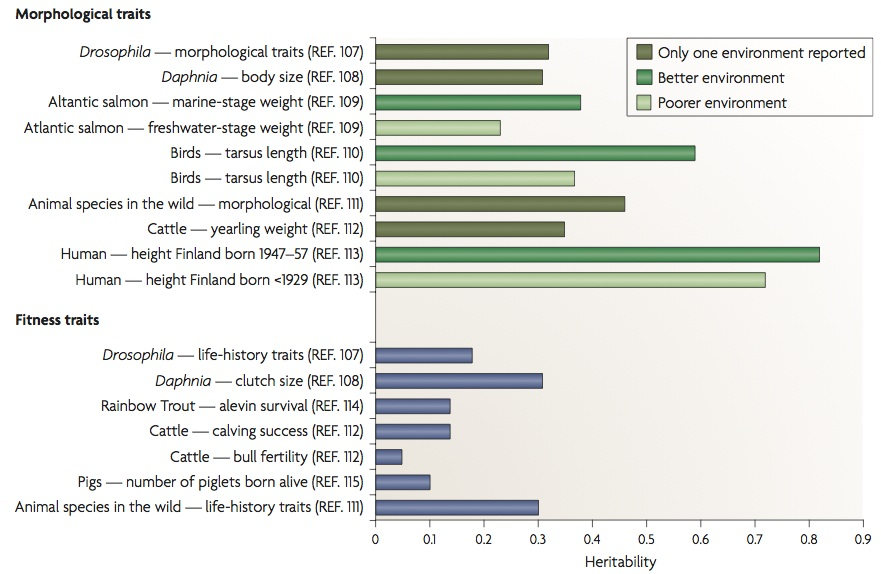
\includegraphics[width=6cm]{visscher2008_heritabiliy.jpg} \\
{\tiny Visscher, 2008}
\end{figure}
\begin{itemize}
\item Fitness related traits have lower heritabilites
\item Additive variance appears to be maintained under selection
\item Response to selection is lower than expected for fitness related traits
\end{itemize}
\end{frame}


\section{Epistasis}
\subsection{}

\begin{frame}{Epistasis}
\begin{definition}
{\color{orange} The effect on the phenotype caused by locus A depends on the genotype at locus B }
%{\tiny \color{white} \newline - Carlborg and Haley 2004 }
\end{definition}
\end{frame}

\begin{frame}{Examples}

\begin{figure}[htb]
 \centering
 \begin{minipage}[c]{0.38\textwidth}
  \centering
{\tiny
\begin{tabular}{cccc}
& AA & Aa & aa \\\hline
BB & $2\alpha + 2\beta$ & $\alpha + 2\beta$ & $2\beta$ \\
Bb & $2\alpha + \beta$ & $\alpha + \beta$ & $\beta$ \\
bb & $2\alpha$ & $\alpha$ & $0$ \\
&&&\\
\multicolumn{4}{l}{Additive + additive (not epistatic)}\\

\end{tabular} }
 \end{minipage}
 \begin{minipage}[c]{0.38\textwidth}
 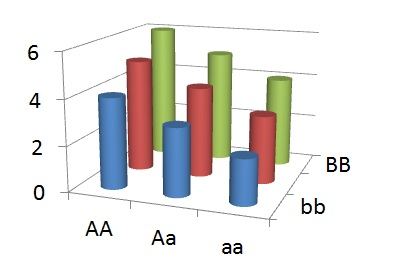
\includegraphics[width=\textwidth]{additive.jpg}
 \end{minipage}
 \end{figure}

\begin{figure}[htb]
 \centering
 \begin{minipage}[c]{0.38\textwidth}
   \centering
{\tiny
\begin{tabular}{cccc}
& AA & Aa & aa \\\hline
BB & $\alpha$ & $\alpha$ & $\alpha$ \\
Bb & $\alpha$ & $\alpha$ & $\alpha$ \\
bb & $\alpha$ & $\alpha$ & $\beta$ \\
&&&\\
\multicolumn{4}{l}{Canalisation (epistatic)}\\
\end{tabular} }
 \end{minipage}
 \begin{minipage}[c]{0.38\textwidth}
 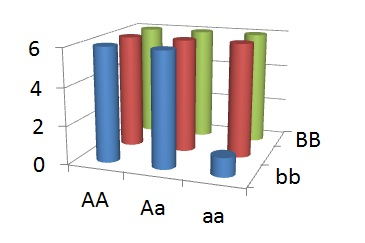
\includegraphics[width=\textwidth]{canalisation.jpg}
 \end{minipage}
\end{figure}
\end{frame}

\begin{frame}{Two dimensional GWAS}
\begin{center}
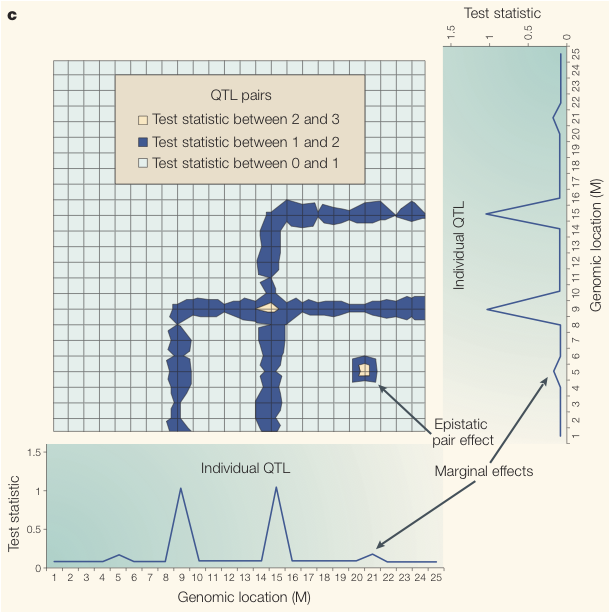
\includegraphics[width=7cm]{2dscan.png} \\
{\tiny Carlborg 2004}
\end{center}
\end{frame}

\begin{frame}{Impact of LD on observed variance}
\begin{center}
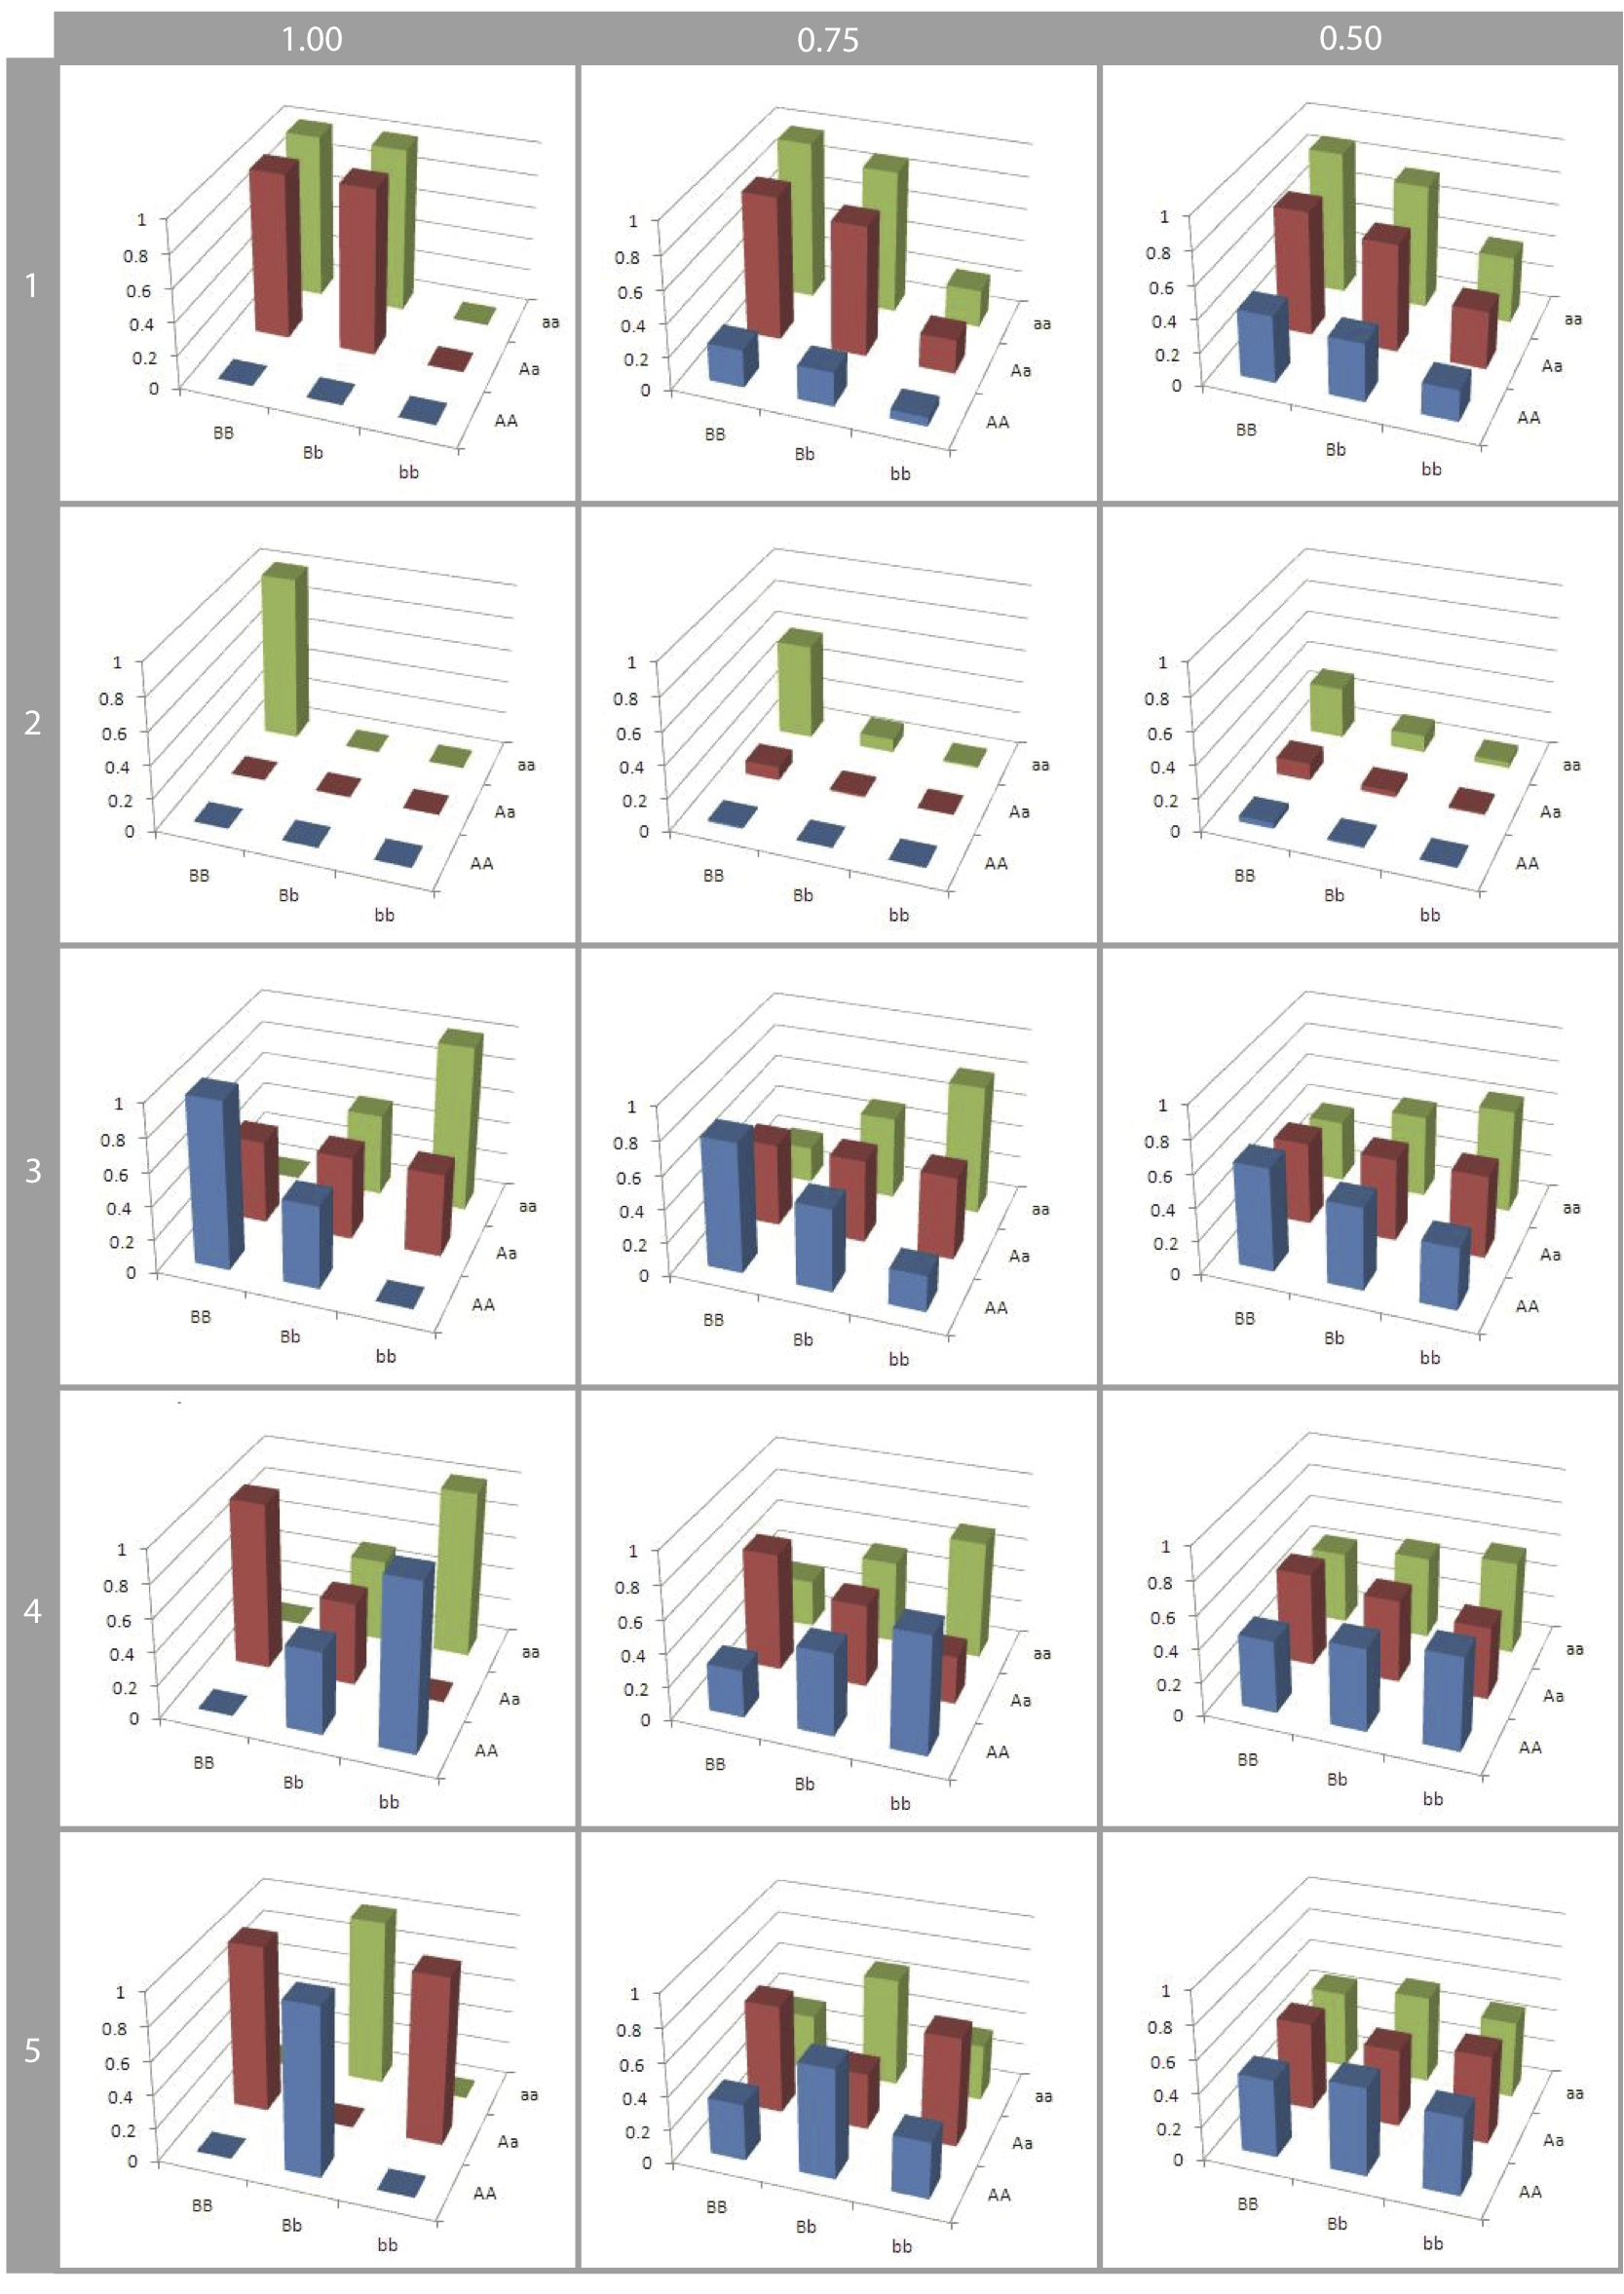
\includegraphics[width=5cm]{gpmaps_ld.png} \\
\end{center}
\end{frame}

\begin{frame}{Can epistasis maintain additive variance?}
\begin{itemize}
\item Hypothesis: Epistasis can maintain additive variance better than purely additive effects
\item How can maintained additive variance be detected most effectively?
\item What is the impact of low LD between causal variants and observed SNPs?
\end{itemize}
\end{frame}


\begin{frame}{Epistatic patterns}
\begin{center}
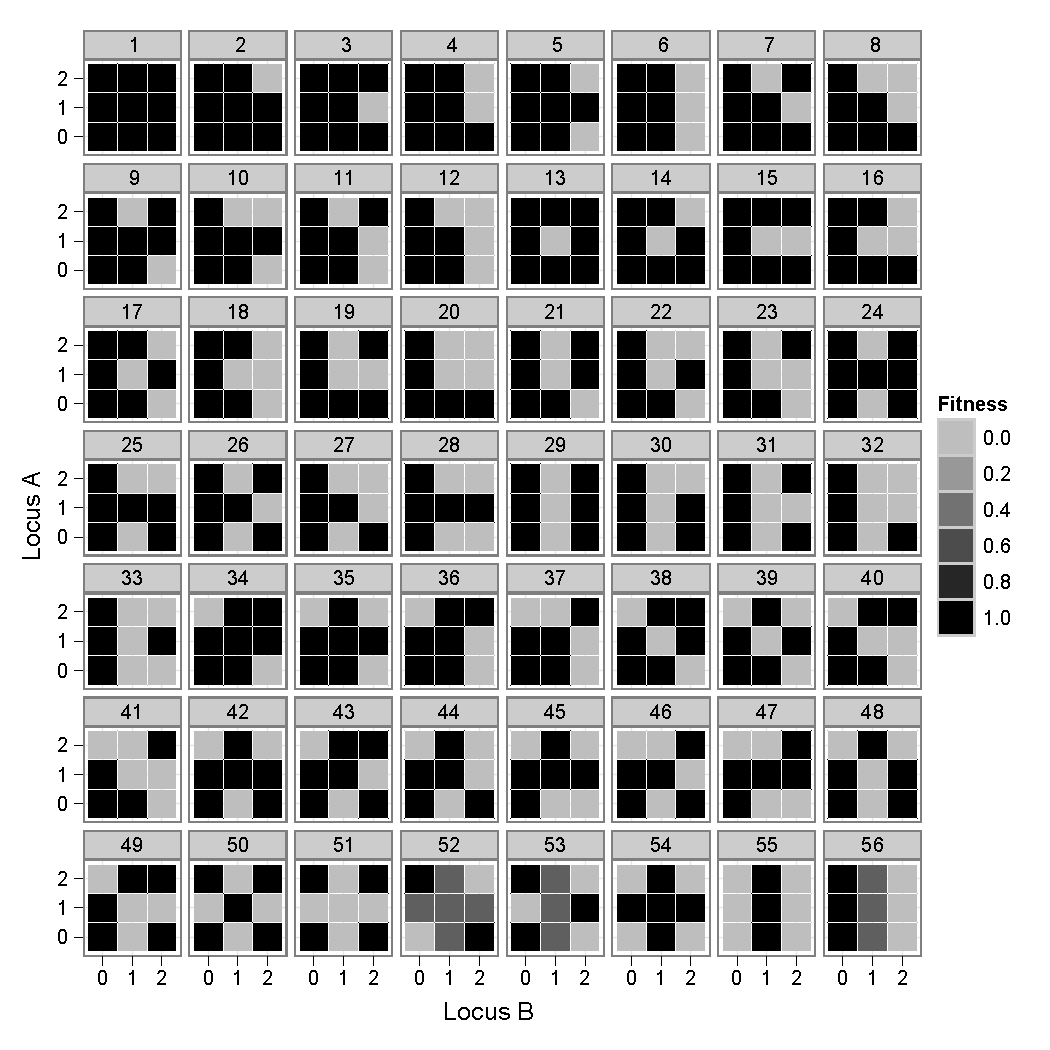
\includegraphics[width=8cm]{sup_gpmaps.pdf}
\end{center}
\end{frame}

\begin{frame}{Allele frequency trajectories}
\begin{center}
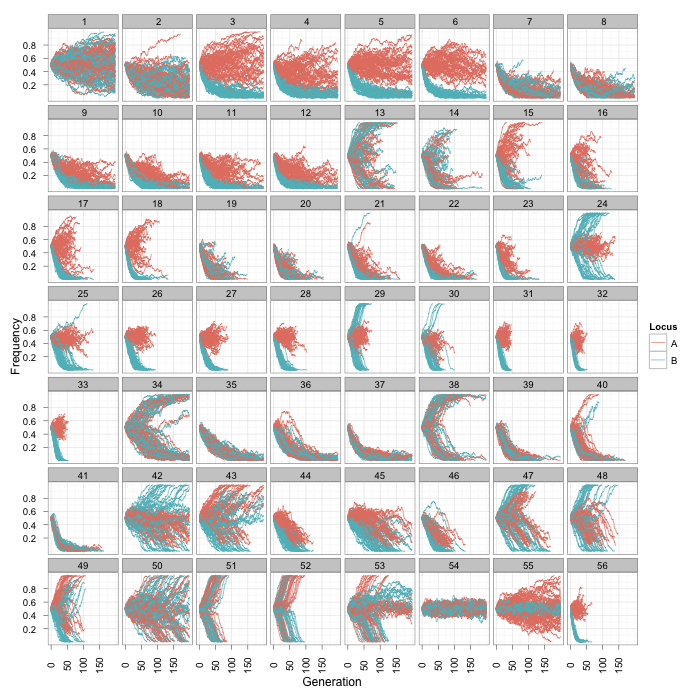
\includegraphics[width=8cm]{sup_allelefreq_sim.png}
\end{center}
\end{frame}

\begin{frame}{Changes in variance under selection}
\begin{center}
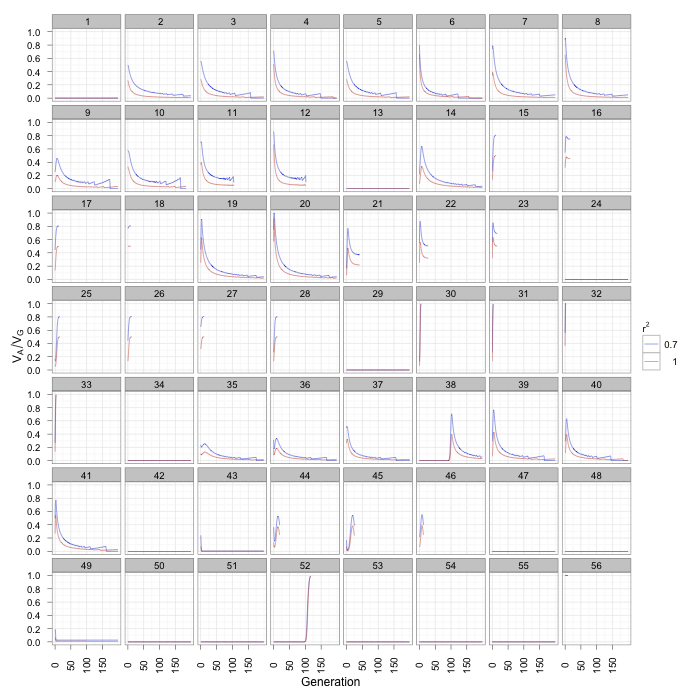
\includegraphics[width=8cm]{sup_propadditive_det.png}
\end{center}
\end{frame}

\begin{frame}{Power to detect evolutionarily persistant variants}

\begin{columns}[c]

\column{.7\textwidth}

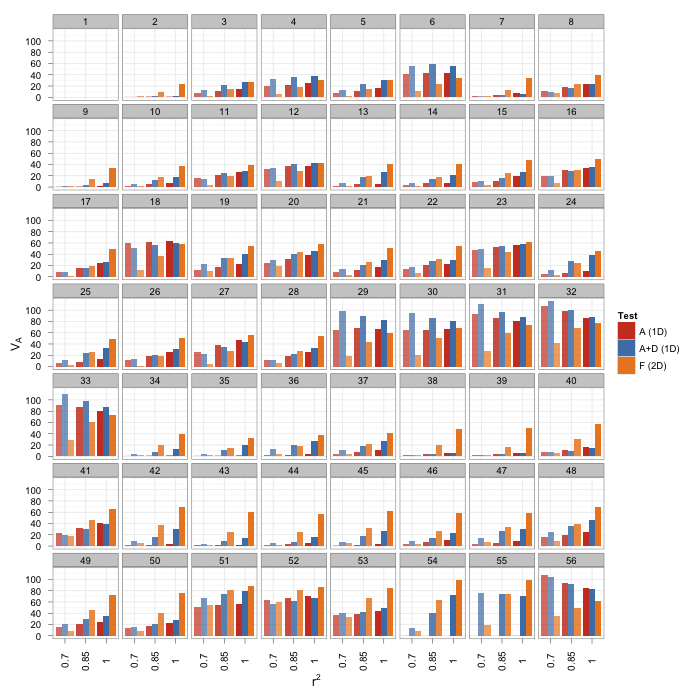
\includegraphics[width=8cm]{sup_heritbars_sim.png}

\column{.3\textwidth}

When LD between causal variants and observed SNPs is high, 2D scan is most powerful for 46/54 non-additive patterns

\end{columns}
\end{frame}



\begin{frame}{Can epistasis maintain additive variance?}
\begin{itemize}
\item Hypothesis: Epistasis can maintain additive variance better than purely additive effects
\begin{itemize}
\item Yes, to a much greater extent
\end{itemize}
\item How can maintained additive variance be detected most effectively?
\begin{itemize}
\item 2 dimensional exhaustive searches
\end{itemize}
\item What is the impact of low LD between causal variants and observed SNPs?
\begin{itemize}
\item Upwards bias in reporting additive effects
\end{itemize}
\end{itemize}
\end{frame}



\begin{frame}{The paradox}
\begin{columns}[c]
\column{.5\textwidth}
\begin{itemize}
\item Epistasis can contribute towards the maintenance and observation of additive genetic variance
\item To find the missing additive variance, search for epistatic effects
\end{itemize}
\column{.5\textwidth} 
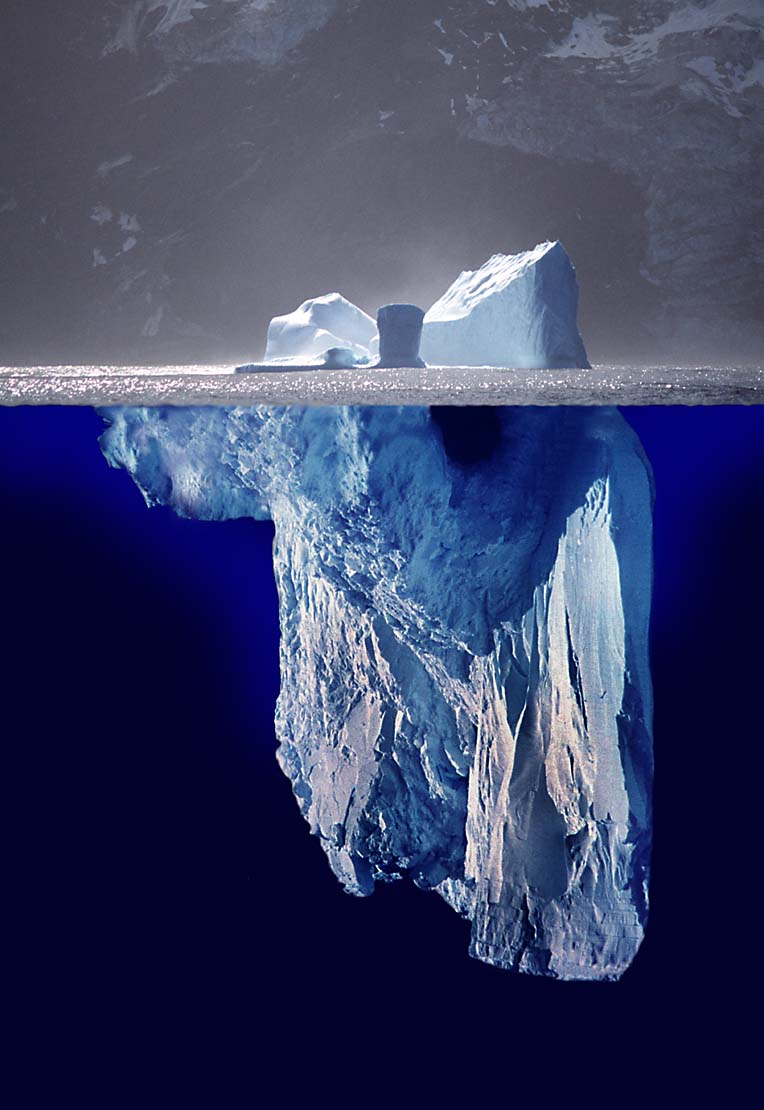
\includegraphics[height=6.5cm]{iceberg.jpg} \\
\end{columns}
\end{frame}


\section{Computational solutions}
\subsection{}

\begin{frame}{The problem}
Number of interactions: \\
\begin{equation}
n(n-1) / 2 \nonumber
\end{equation}
500000 SNPs $\rightarrow$ 125 billion interactions \\
\begin{itemize}
\item PLINK performs 5000 tests per second $\rightarrow$ 3 years
\item FastEpistasis performs 36000 tests per second $\rightarrow$ 5 months
\item Optimised C code 125000 tests per second $\rightarrow$ 6 weeks
\item Parallelised on 8-core CPU $\rightarrow$ 5 days
\end{itemize}
\end{frame}


\begin{frame}{CPUs and hitting the `power wall'}
\begin{itemize}
\item All electrical power consumed eventually radiates as heat
\item Processor speed requires more power to improve
\begin{itemize}
\item Increased heat
\item Increased circuit resistance
\item Instability
\end{itemize}
\end{itemize}
\end{frame}

\begin{frame}{CPU limits}
\begin{center}
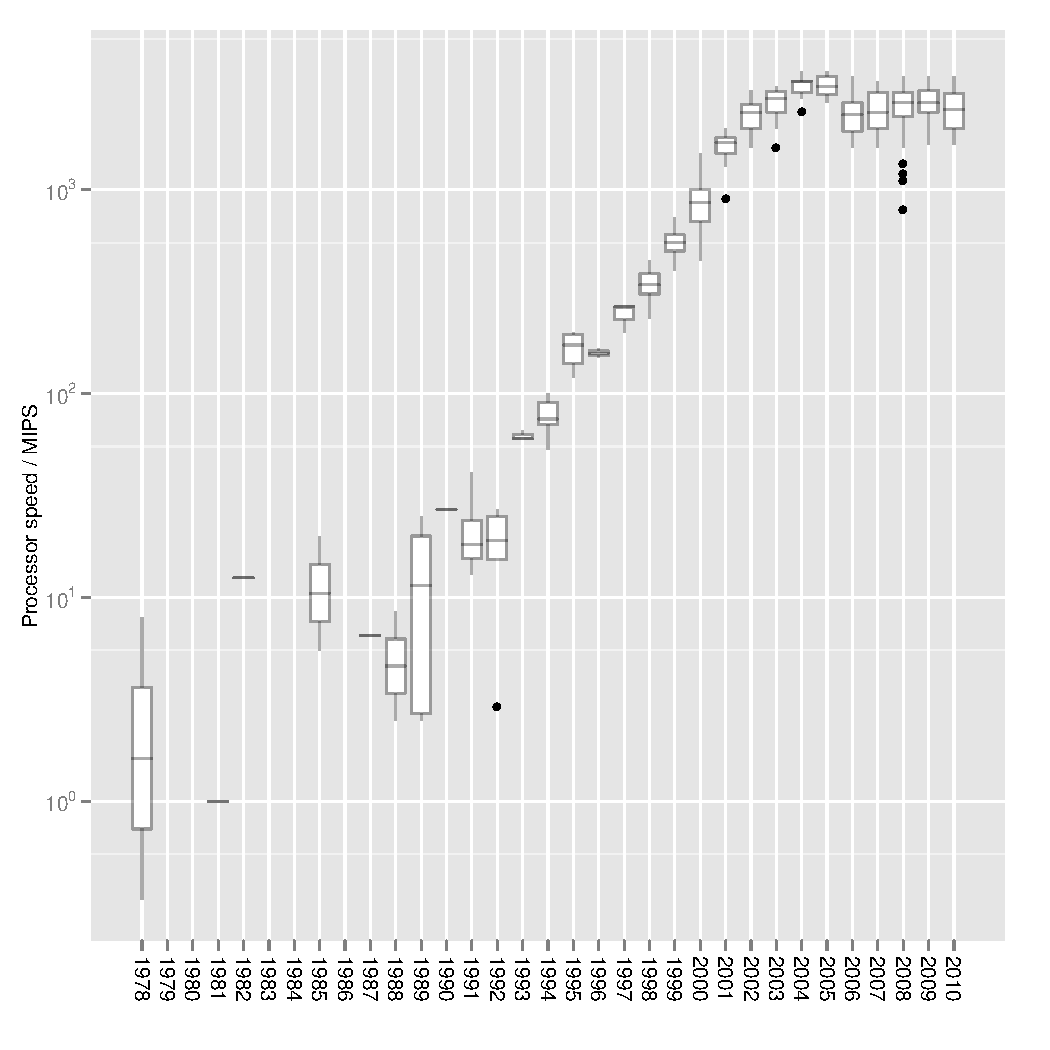
\includegraphics[height=7cm]{clockspeed.pdf}
\end{center}
\end{frame}

\begin{frame}{CPU limits}
\begin{center}
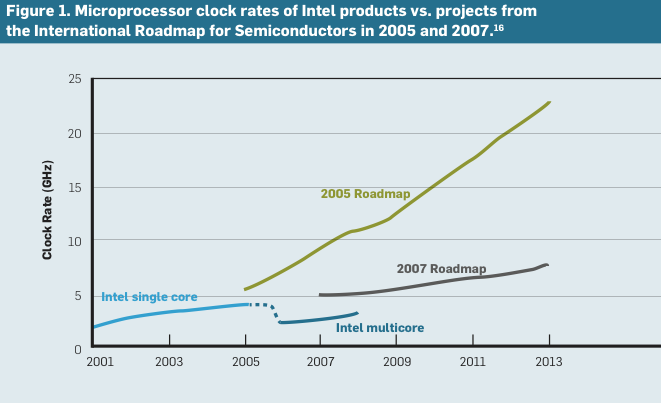
\includegraphics[height=6cm]{clockrates.png}
\end{center}
\end{frame}

\begin{frame}{Graphics Cards}
\begin{itemize}
\item Revenue of video game industry $>$ Hollywood film industry
\item Better games require better hardware
\begin{itemize}
\item Finer pixels rendered faster
\item Physics engines
\item Easily obtained by having many simple cores
\end{itemize}
\item Consumer level graphics cards have hundreds of very simple cores
\item Ideal for geometric parallelisation problems in science
\item Use OpenCL API to communicate with graphics cards

\end{itemize}
\end{frame}


\begin{frame}{Chip structures}
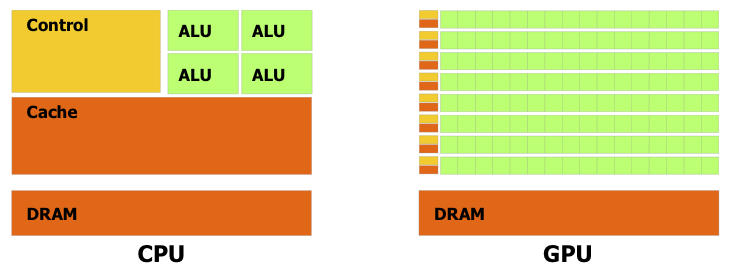
\includegraphics[height=2.5cm]{cpugpu.png}
\begin{itemize}
\item Many cores that can process data simultaneously
\item But all the cores are extremely simple
\begin{itemize}
\item Tiny L1 cache
\item Little communication between cores
\item Each core is relatively slow
\item Cores are divided into local groups, all of which must do the same thing
\end{itemize}

\end{itemize}
\end{frame}


\begin{frame}{GPU speeds}
\begin{center}
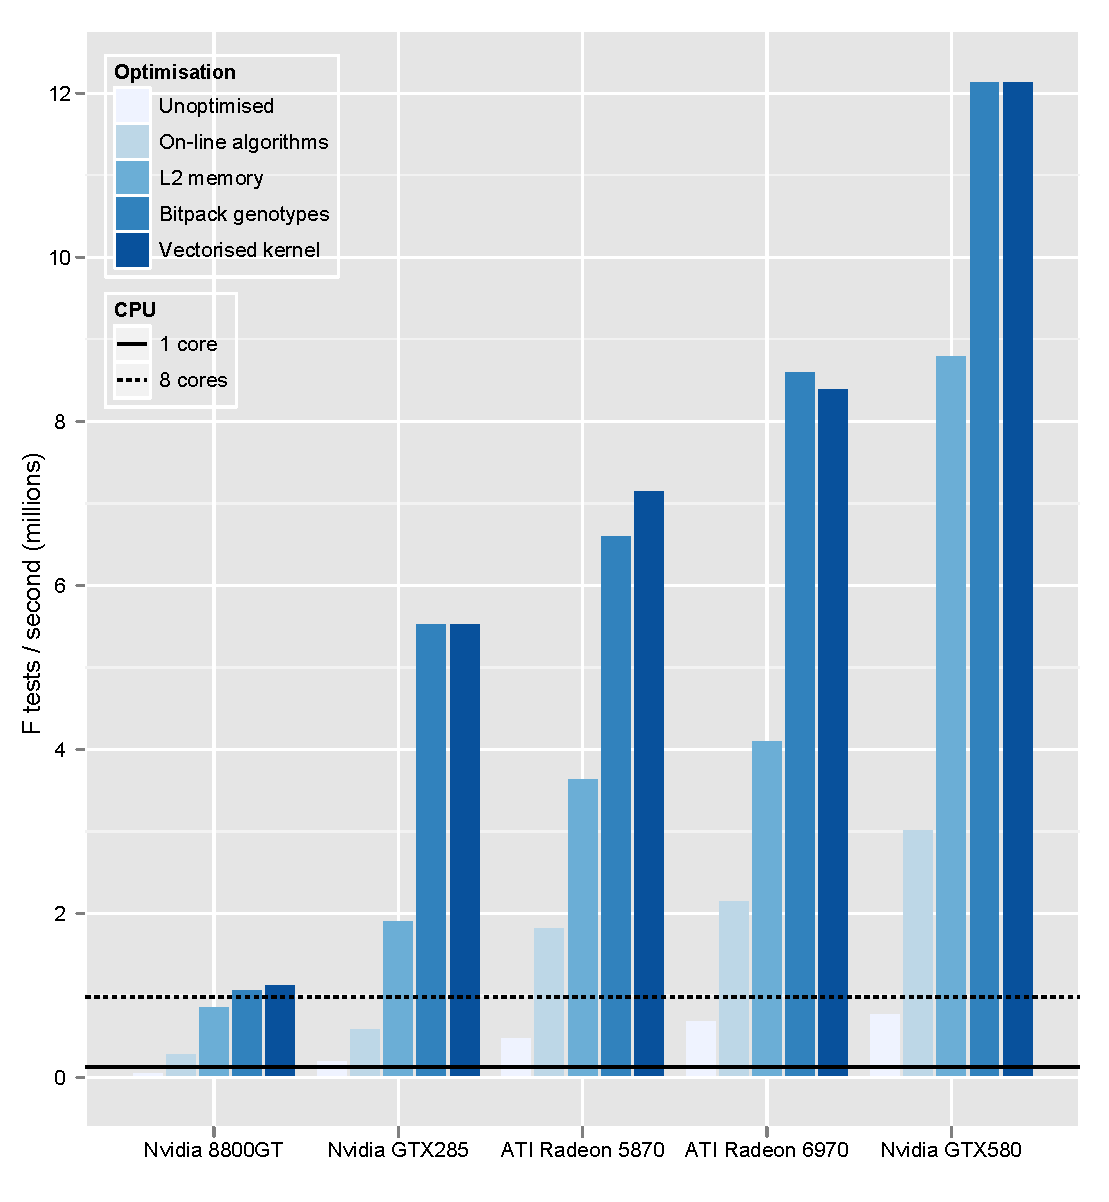
\includegraphics[height=7cm]{gpuoptimisation.pdf}
\end{center}
\end{frame}

\begin{frame}{epiGPU}
\begin{itemize}
\item http://sourceforge.net/projects/epigpu/
\item Free
\item Open source
\item Windows, Mac, Linux
\item NVIDIA and ATI graphics cards
\end{itemize}
\end{frame}


% mention epiGPU

\section{Thresholds}
\subsection{}

\begin{frame}{Multiple testing}
\begin{definition}
{\color{orange} Frequentist $p$-value: The probability of obtaining a test statistic at least as extreme as the one that was actually observed, assuming that the null hypothesis is true.}
\end{definition}
\begin{itemize}
\item \emph{e.g.} If 20 independent tests are performed then would expect one true null to have a $p$-value $\leq 0.05$.
\item So if significance with a false positive rate of $\alpha = 0.05$ is desired, then the threshold for the family of tests should be adjusted to $\alpha_{F} = 0.05 / 20 = 0.0025$.
\item 500000 SNPs being tested $\rightarrow \alpha_{F} = 0.05 / 500000 = 1 \times 10^{-7}$
\item Epistasis $\rightarrow \alpha_{F} = \frac{0.05}{n(n-1)/2} \approx 4 \times 10^{-13}$
\end{itemize}
\end{frame}

\begin{frame}{The curse of dimensionality}
As the dimensionality of the search increases the background noise drowns out all real biological signals
\end{frame}

\begin{frame}{Linkage disequilibrium}
\begin{center}
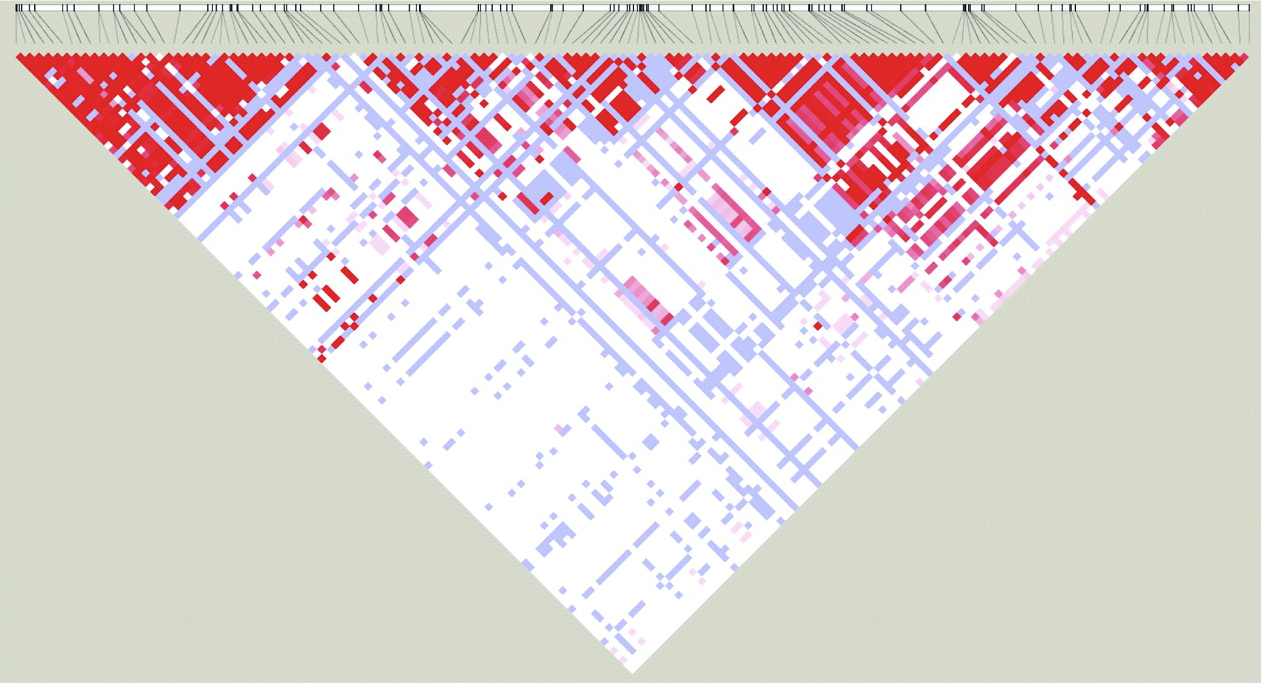
\includegraphics[width=10cm]{ld.png}
\end{center}
\begin{itemize}
\item SNPs are correlated $\rightarrow$ tests are not independent
\item Bonferroni correction is overly stringent
\end{itemize}
\end{frame}

\begin{frame}{Permutation analysis}
What is the \emph{effective} number of multiple tests that are being performed? (Churchill 1994)
\begin{center}
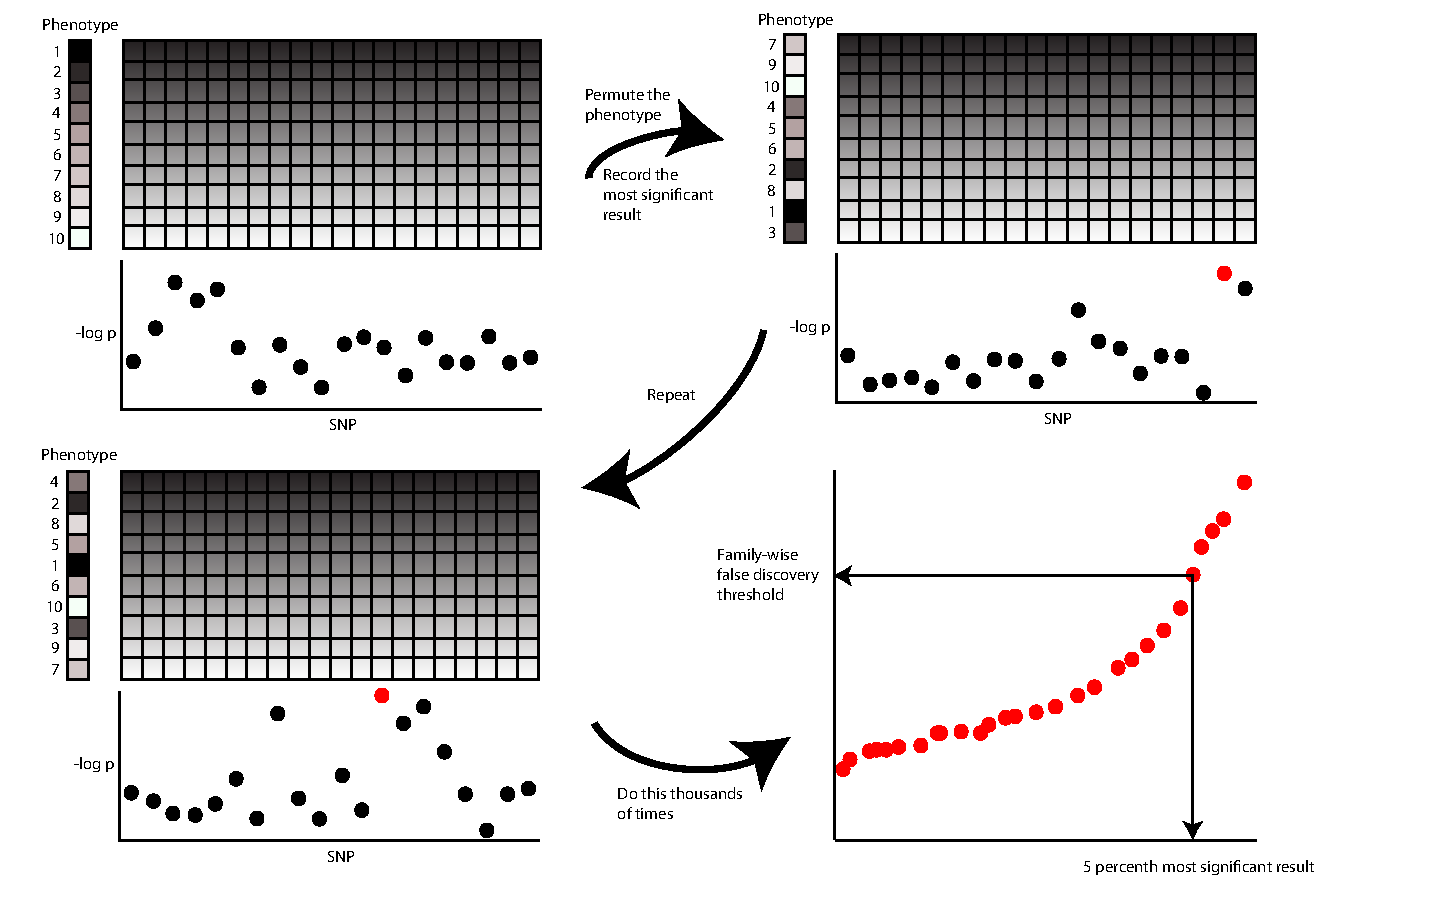
\includegraphics[width=10cm]{permutationanalysis.pdf}
\end{center}
\end{frame}

\begin{frame}{What is the correlation structure in a 2D search?}
\begin{center}
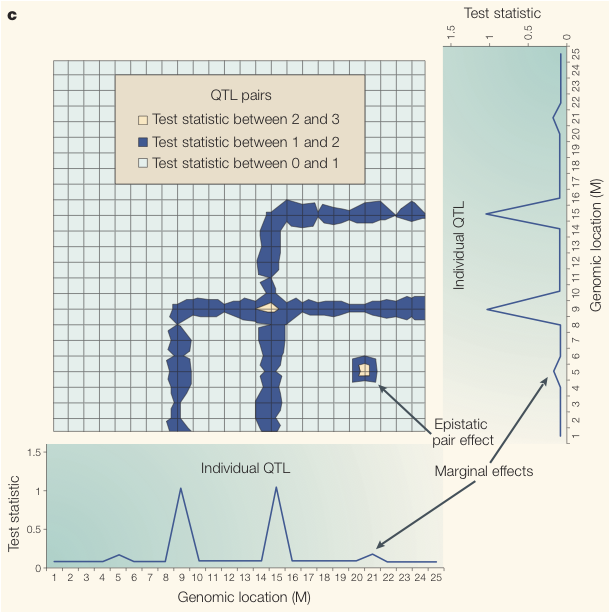
\includegraphics[width=7cm]{2dscan.png} \\
{\tiny Carlborg 2004}
\end{center}
\end{frame}

\begin{frame}{Epistatic permutations}
\begin{itemize}
\item How is the 2D threshold governed by:
\begin{itemize}
\item Number of SNPs being tested
\item Number of individuals in the study?
\end{itemize}
\item Difficult computational challenge
\begin{itemize}
\item Requires cluster of GPUs...
\item ...running for months!
\end{itemize}
\end{itemize}
\end{frame}


\begin{frame}{A general formula for 2D thresholds?}
\begin{equation}
-\log_{10}(p_{T}) = a - a \left ( 
 s_{1} \exp \left ( 
  \frac {\ln(n) } { s_{2} } \right )
 + s_{3} \exp \left (
  \frac{ \ln(M)} {s_{4}} \right ) 
\right )^{-1} \nonumber
\label{eqn:general_threshold}
\end{equation}
\begin{eqnarray}
a & = & 12.68 \nonumber \\
s_{1} & = & 0.0258 \nonumber \\
s_{2} & = & 1.72 \nonumber \\
s_{3} & = & 0.0379 \nonumber \\
s_{4} & = & 2.33. \nonumber
\end{eqnarray}
\end{frame}

\begin{frame}{A general formula for 2D thresholds?}
\begin{center}
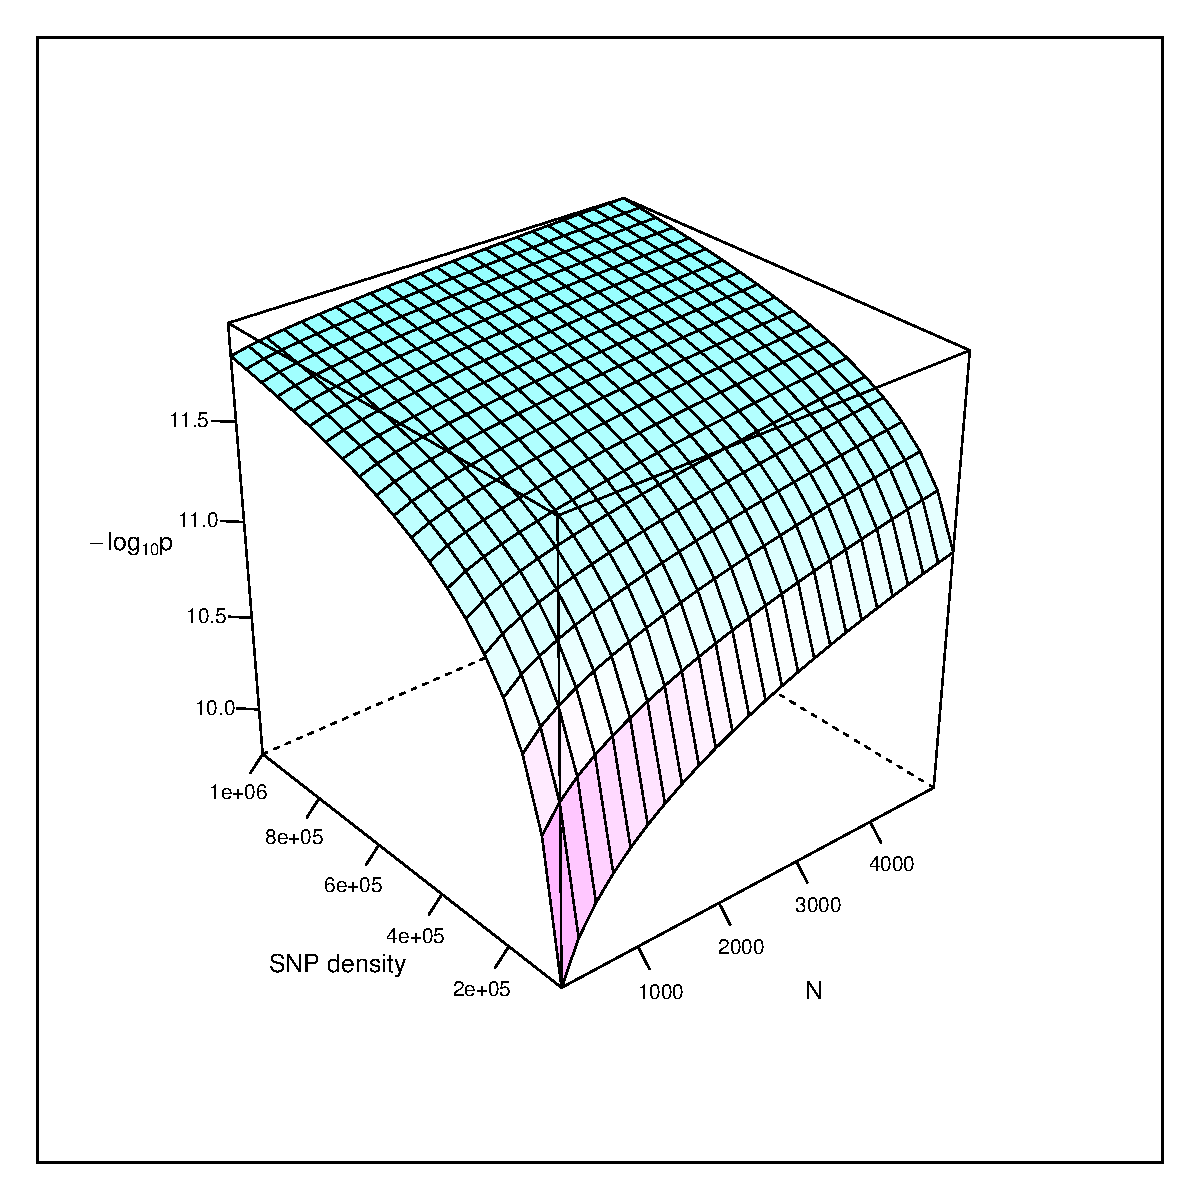
\includegraphics[height=7cm]{threshold_function.pdf}
\end{center}
\end{frame}


\section{2D eQTL}
\subsection{}

\begin{frame}{Are epistatic effects controlling gene expression?}
\begin{itemize}
\item Study design:
\begin{itemize}
\item 846 healthy Australian adults
\item 546,192 SNPs
\item 5380 gene expression probes from whole blood
\end{itemize}
\item Plan:
\begin{itemize}
\item Do exhaustive search for 2 locus epistasis for each probe
\item Parallelise search across 100x GPU cluster
\end{itemize}
\end{itemize}
\end{frame}

\begin{frame}{Thresholds}
\begin{itemize}
\item 1641 complete scans were performed on permuted phenotype
\item Threshold predicted to be: \textbf{11.648}
\item Empirical estimate: \textbf{11.632}
\item Average correlation between 5380 probes: \textbf{0.265}
\item Overall threshold: $-\log_{10}p =$ \textbf{16.5}
\end{itemize}
\end{frame}

\begin{frame}{Very preliminary results}
\begin{itemize}
\item Is there much non-additive variance?
\item 71 probes have significant eQTLs after filtering for:
\begin{itemize}
\item Threshold of 16.5
\item Additive variance $\leq$ 60\% of total genetic variance
\item Relatively common SNPs (must have samples for all 9 genotype classes)
\item No LD between interacting SNPs
\end{itemize}
\item Total of 140 significant independent loci
\end{itemize}
\end{frame}

\begin{frame}{Very preliminary results}
\begin{itemize}
\item Proportion of the phenotypic variance explained:
\begin{itemize}
\item Total genetic: range 8.4\% - 17.1\%
\item Total non-additive: range 3.5\% - 9.2\%
\end{itemize}
\item 14\% cis-cis
\item 69\% cis-trans
\item 17\% trans-trans
\end{itemize}
\end{frame}

\begin{frame}{Some examples}
\begin{center}
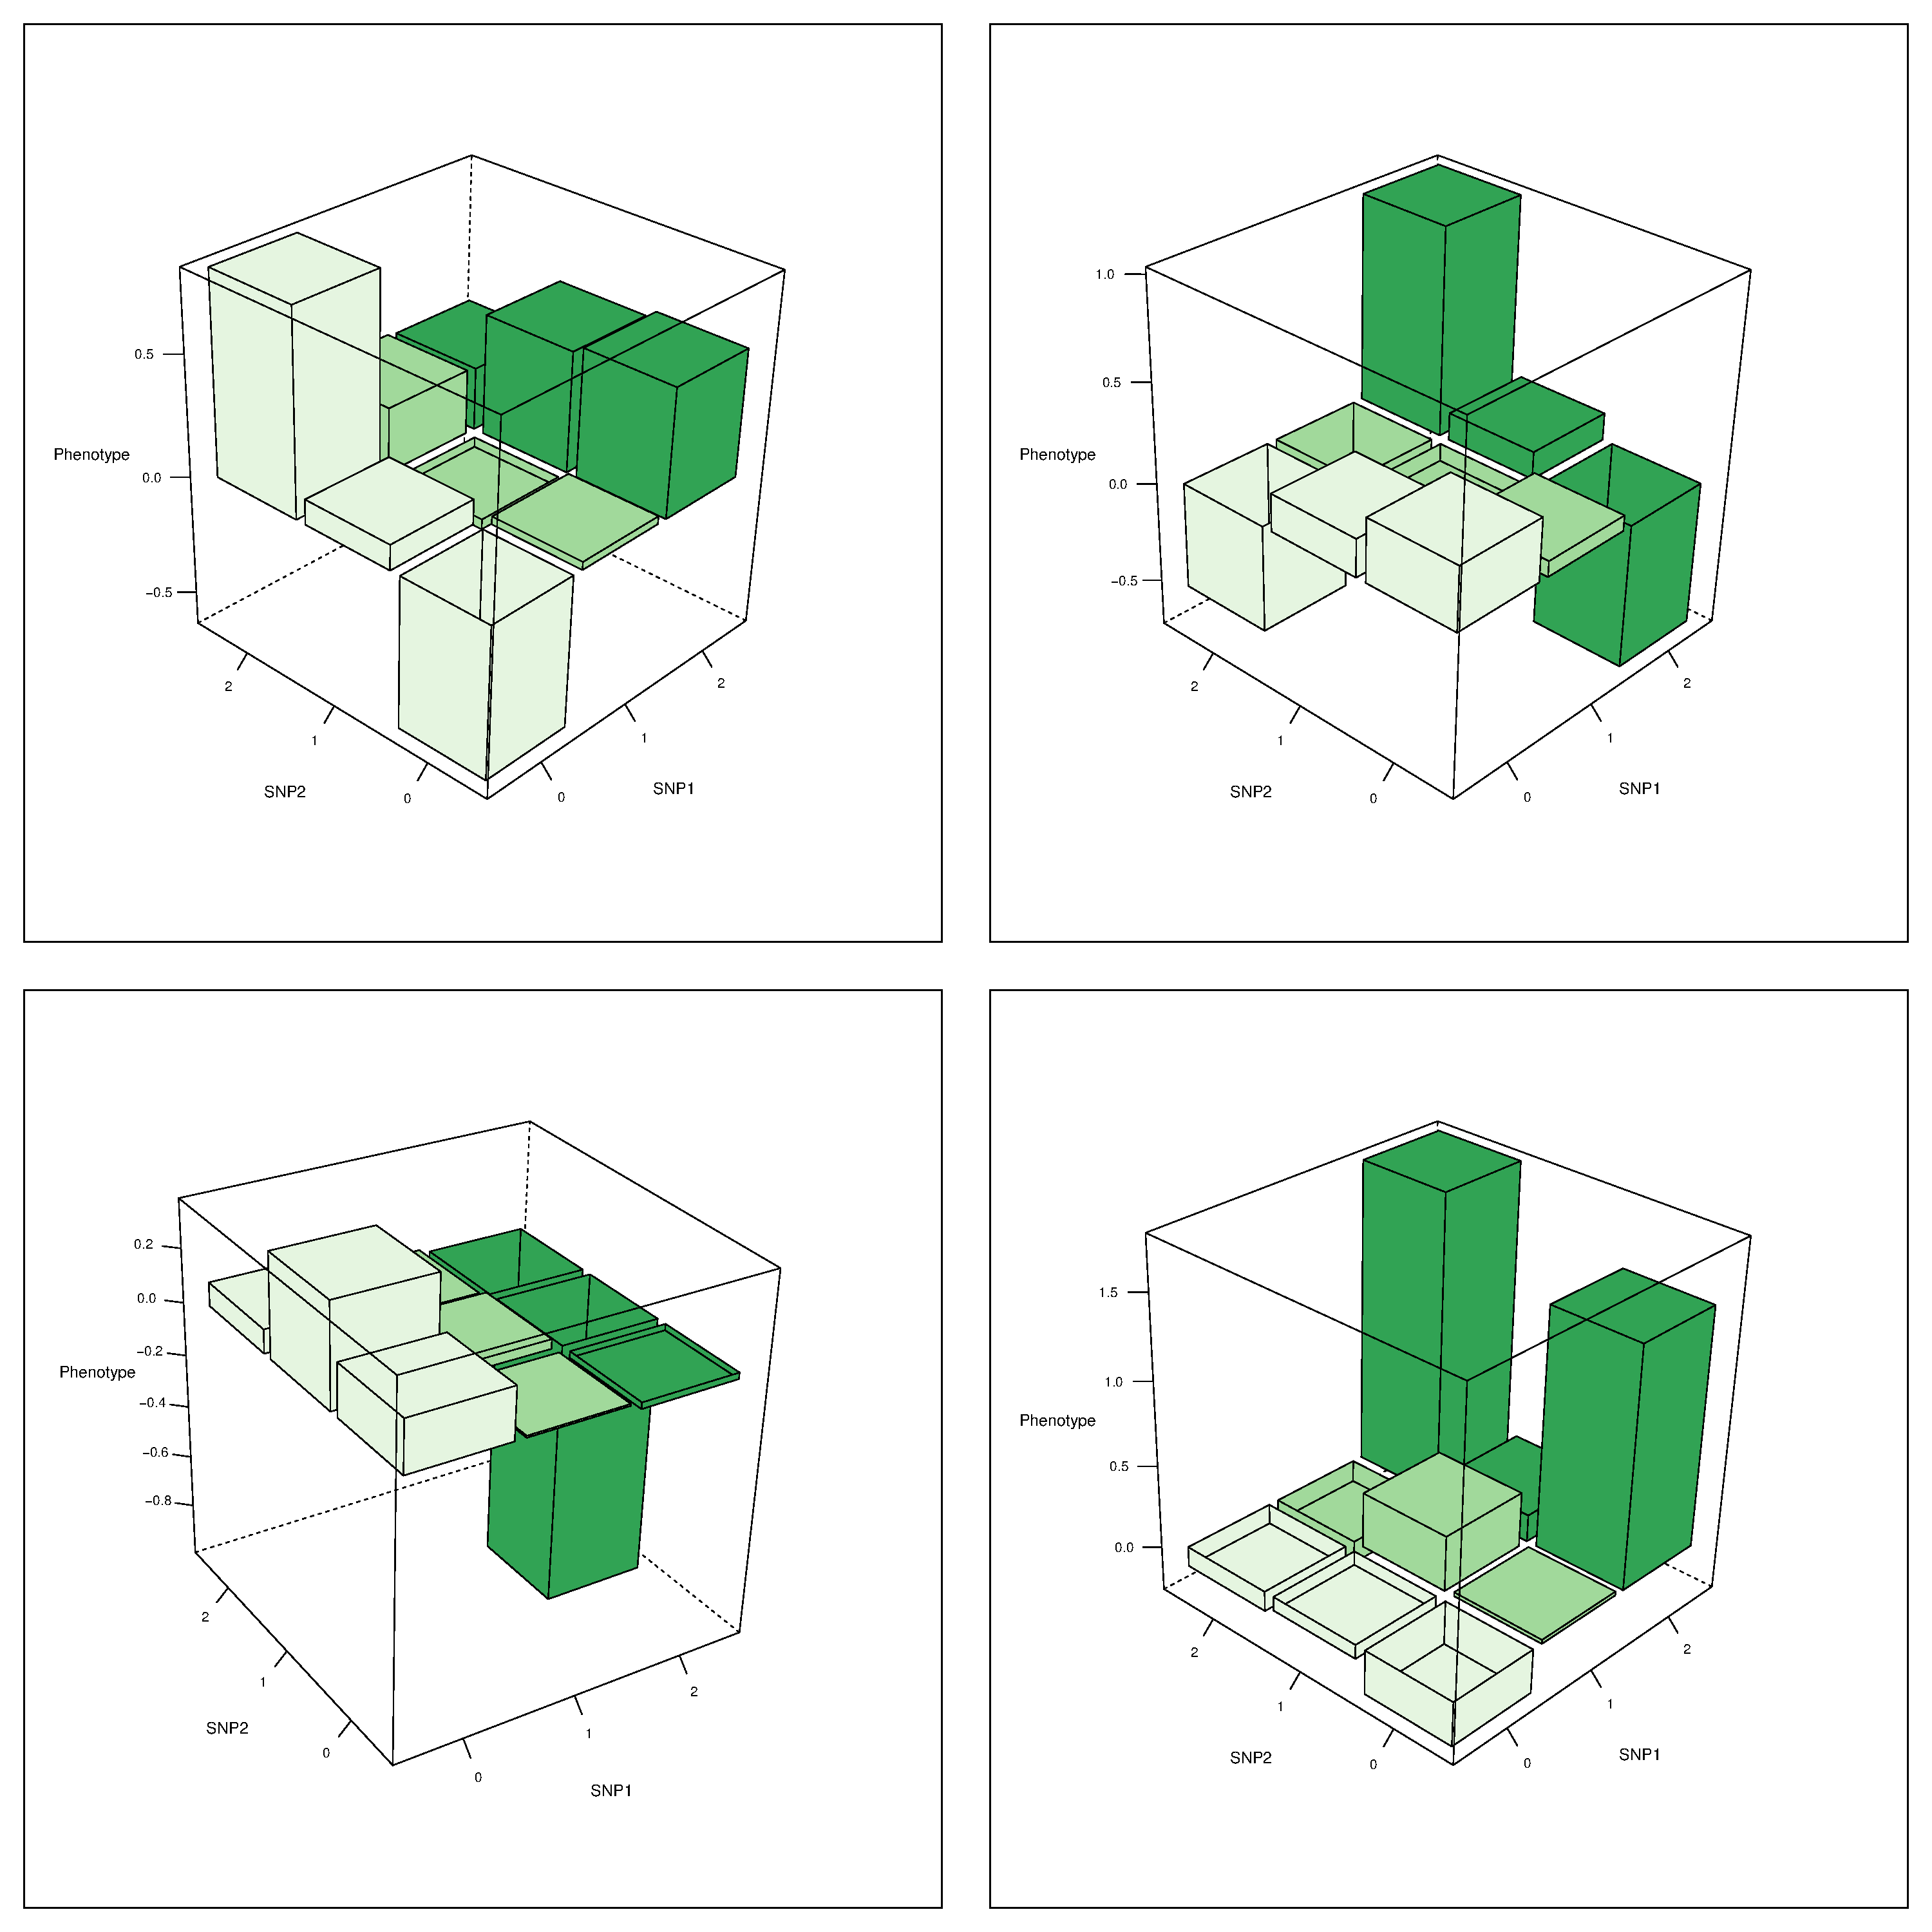
\includegraphics[height=7.5cm]{epistasis_examples}
\end{center}
\end{frame}


\section*{}

\begin{frame}{Acknowledgements}


\begin{columns}[c]

\column{.5\textwidth}

{\tiny
PhD Funding:
\begin{itemize}
\item The Roslin Institute
\item University of Edinburgh
\item Biosciences KTN
\item Monsanto / NCG
\end{itemize}
PhD Supervisors:
\begin{itemize}
\item Chris Haley
\item Sara Knott
\item John Woolliams
\end{itemize}
Important people:
\begin{itemize}
\item Ricardo Pong-Wong
\item Athanasios Theocharidis
\item Wenhua Wei
\end{itemize}
Compute resources
\begin{itemize}
\item ECDF - {\tt eddie}
\item Daresbury Labs - {\tt cseht}
\item IVEC - {\tt fornax}
\end{itemize}
}

\column{.5\textwidth}

{\tiny
Complex Trait Genomics Group

\begin{itemize}
\item Peter Visscher
\item Naomi Wray
\item \textbf{Joseph Powell}
\item Jian Yang
\item Allan Mcrae
\item Anita Goldinger
\item Hong Lee
\item Anna Vinkhuyzen
\item Guo-Bo Chen
\item Beben Benyamin
\item Zong Zhang
\item Enda Byrne
\item Marie-Jo Brion
\item Sven Stringer
\end{itemize}
}

\end{columns}
\end{frame}

\begin{frame}
\centering
Thanks!
\end{frame}


\begin{frame}{Sample size vs 2D threshold}


\begin{equation}
\lim_{n \to \infty} \bar{g} = 9 \nonumber
\end{equation}

\begin{eqnarray}
-\log \left ( f \left (
\frac{
 SS_{W}  (g - 1)^{-1}
}
{  SS_{B} (n - g)^{-1}
}; g - 1, n - g
\right ) \right )
& \propto &
 n \nonumber \\ 
& \propto &
SS_{W} / (SS_{W} + SS_{B}) \nonumber \\
& \propto &
-\log(g) \nonumber
\label{eq:ftest_n}
\end{eqnarray}

\end{frame}



\begin{frame}{GP maps from genetic algorithm}
\begin{center}
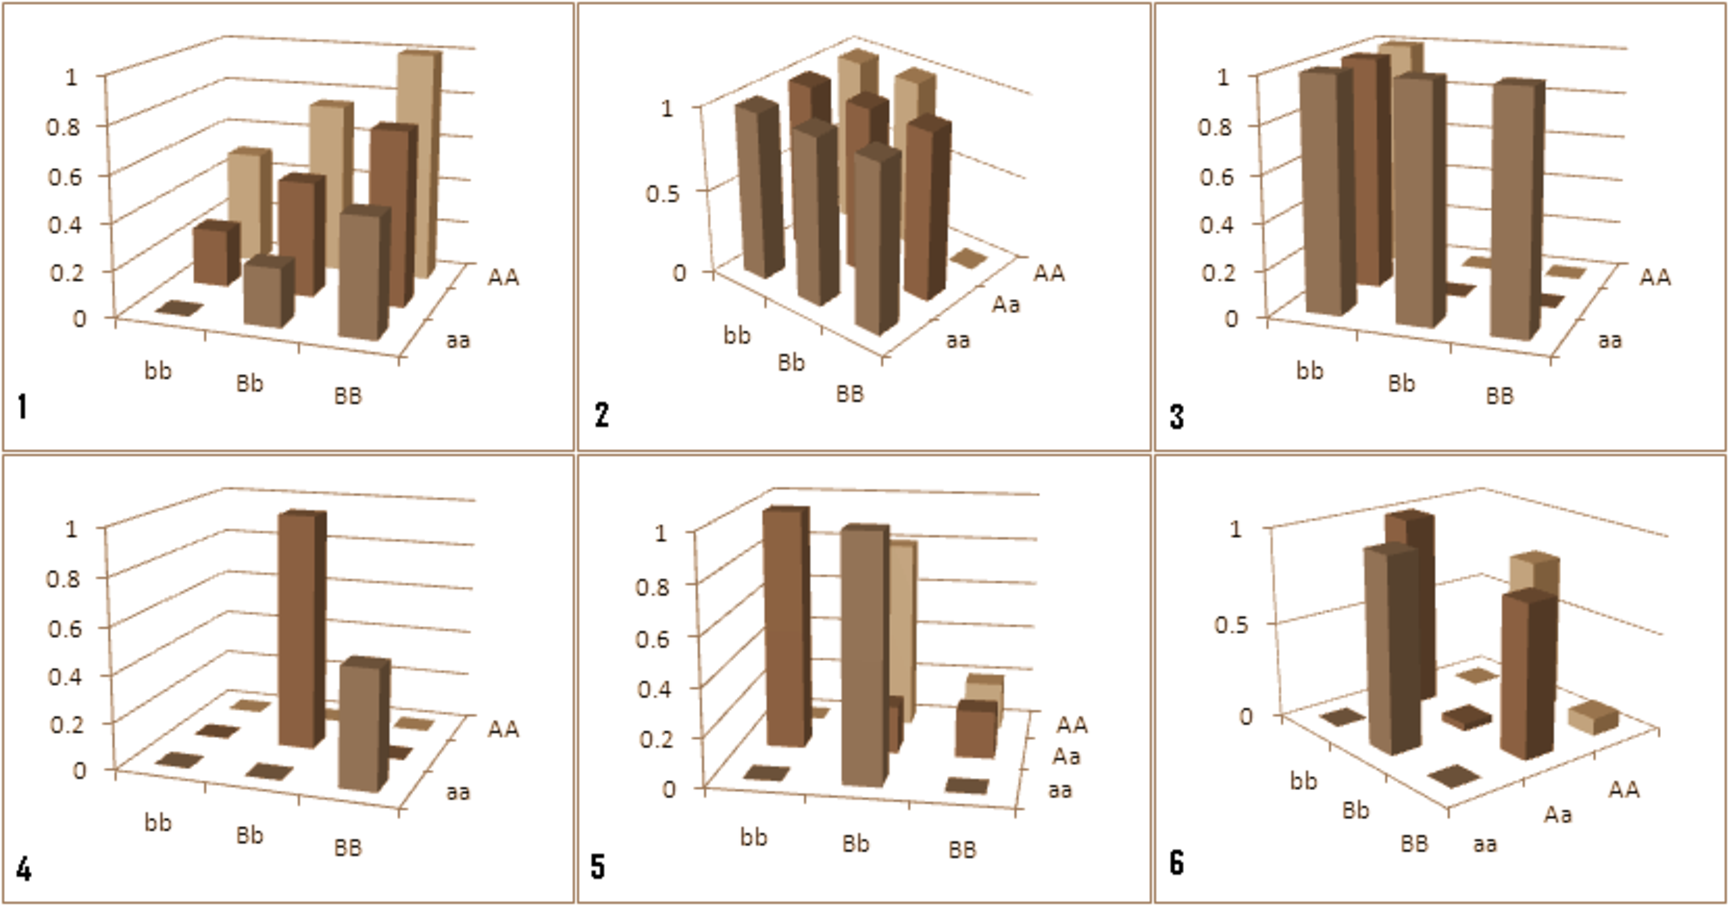
\includegraphics[width=8cm]{gpmaps2.pdf}
\end{center}
\end{frame}

\begin{frame}{Allele frequency trajectories}
\begin{center}
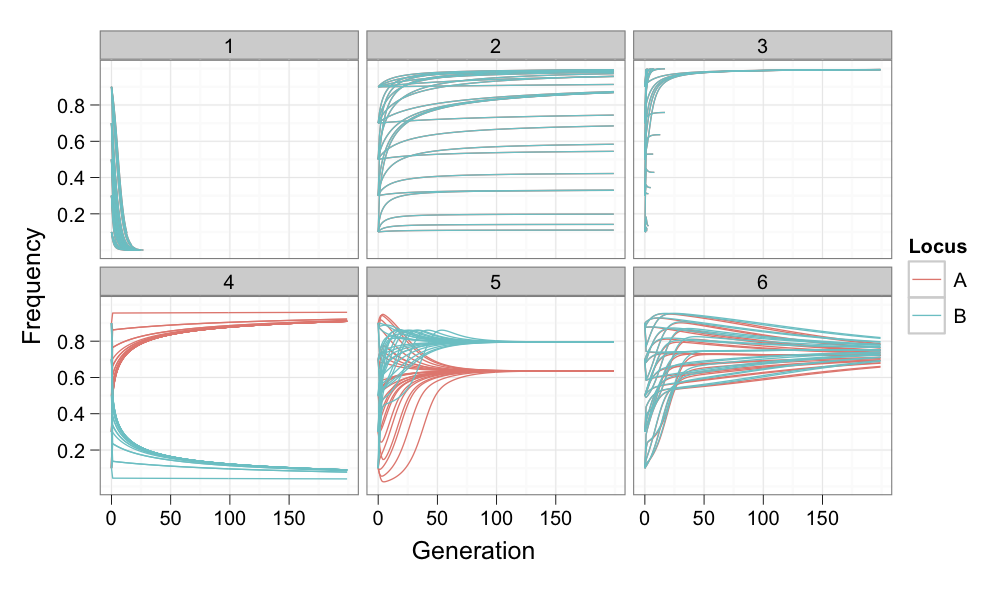
\includegraphics[width=8cm]{allelefreq_det.png}
\end{center}
\end{frame}

\begin{frame}{Changes in variance under selection}
\begin{center}
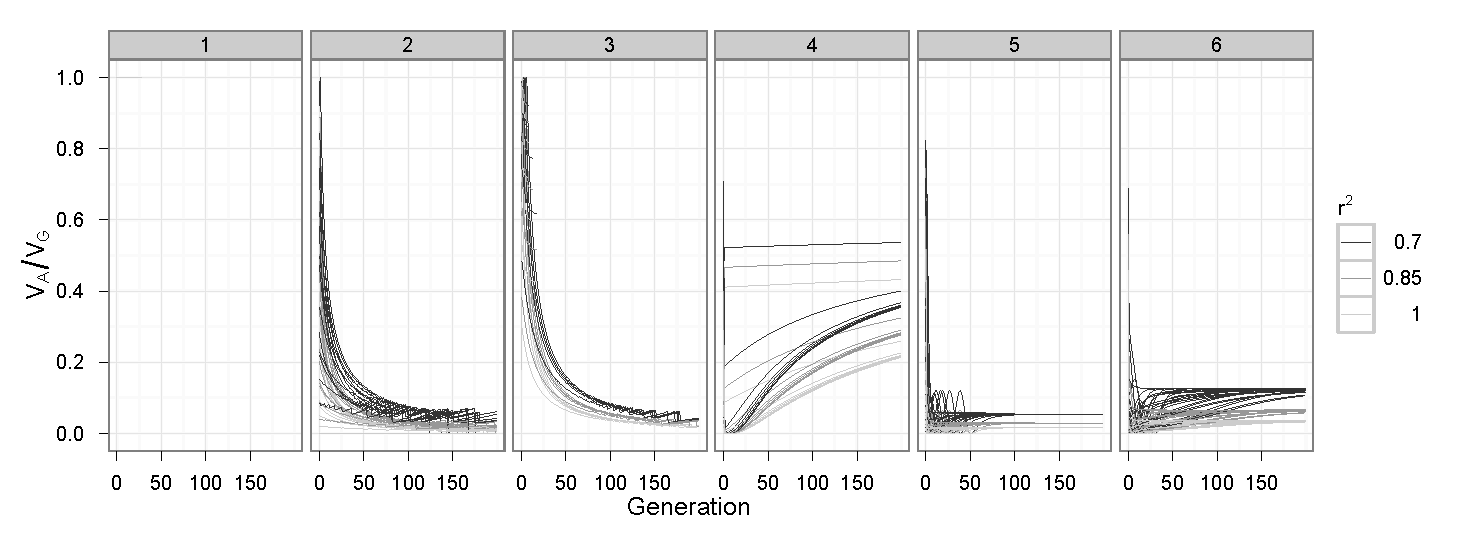
\includegraphics[width=10cm]{propadditive_det_grey.pdf} \\
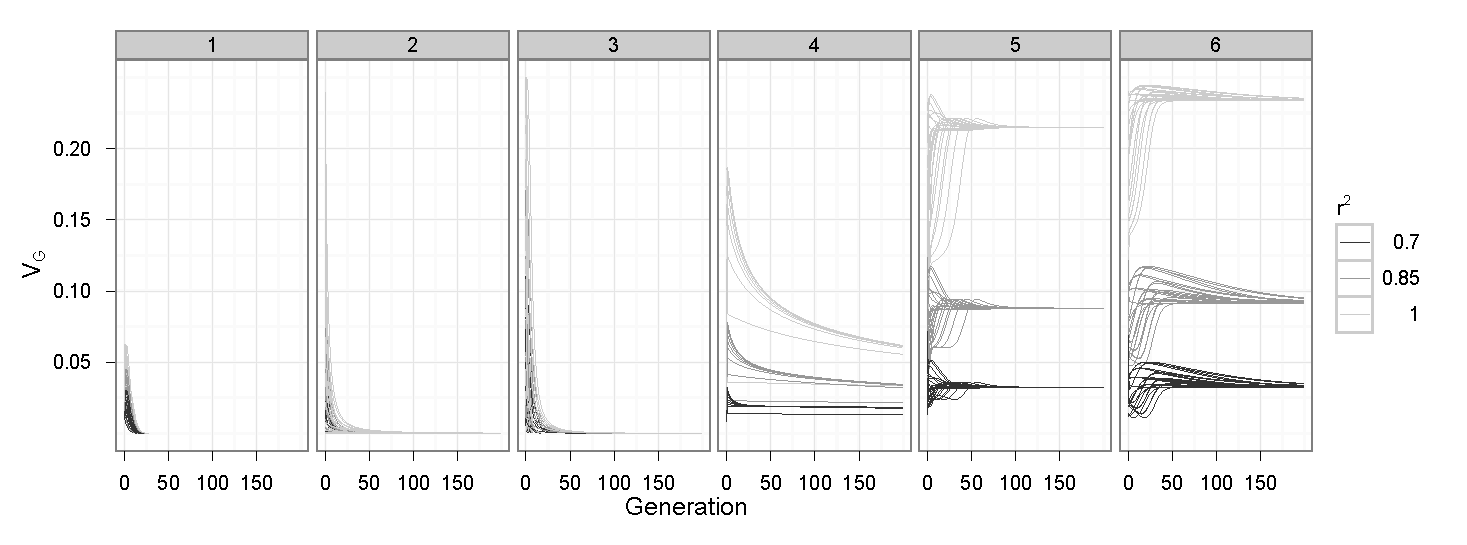
\includegraphics[width=10cm]{Vg_det_grey.pdf}
\end{center}
\end{frame}

\begin{frame}{Power studies}
\begin{center}
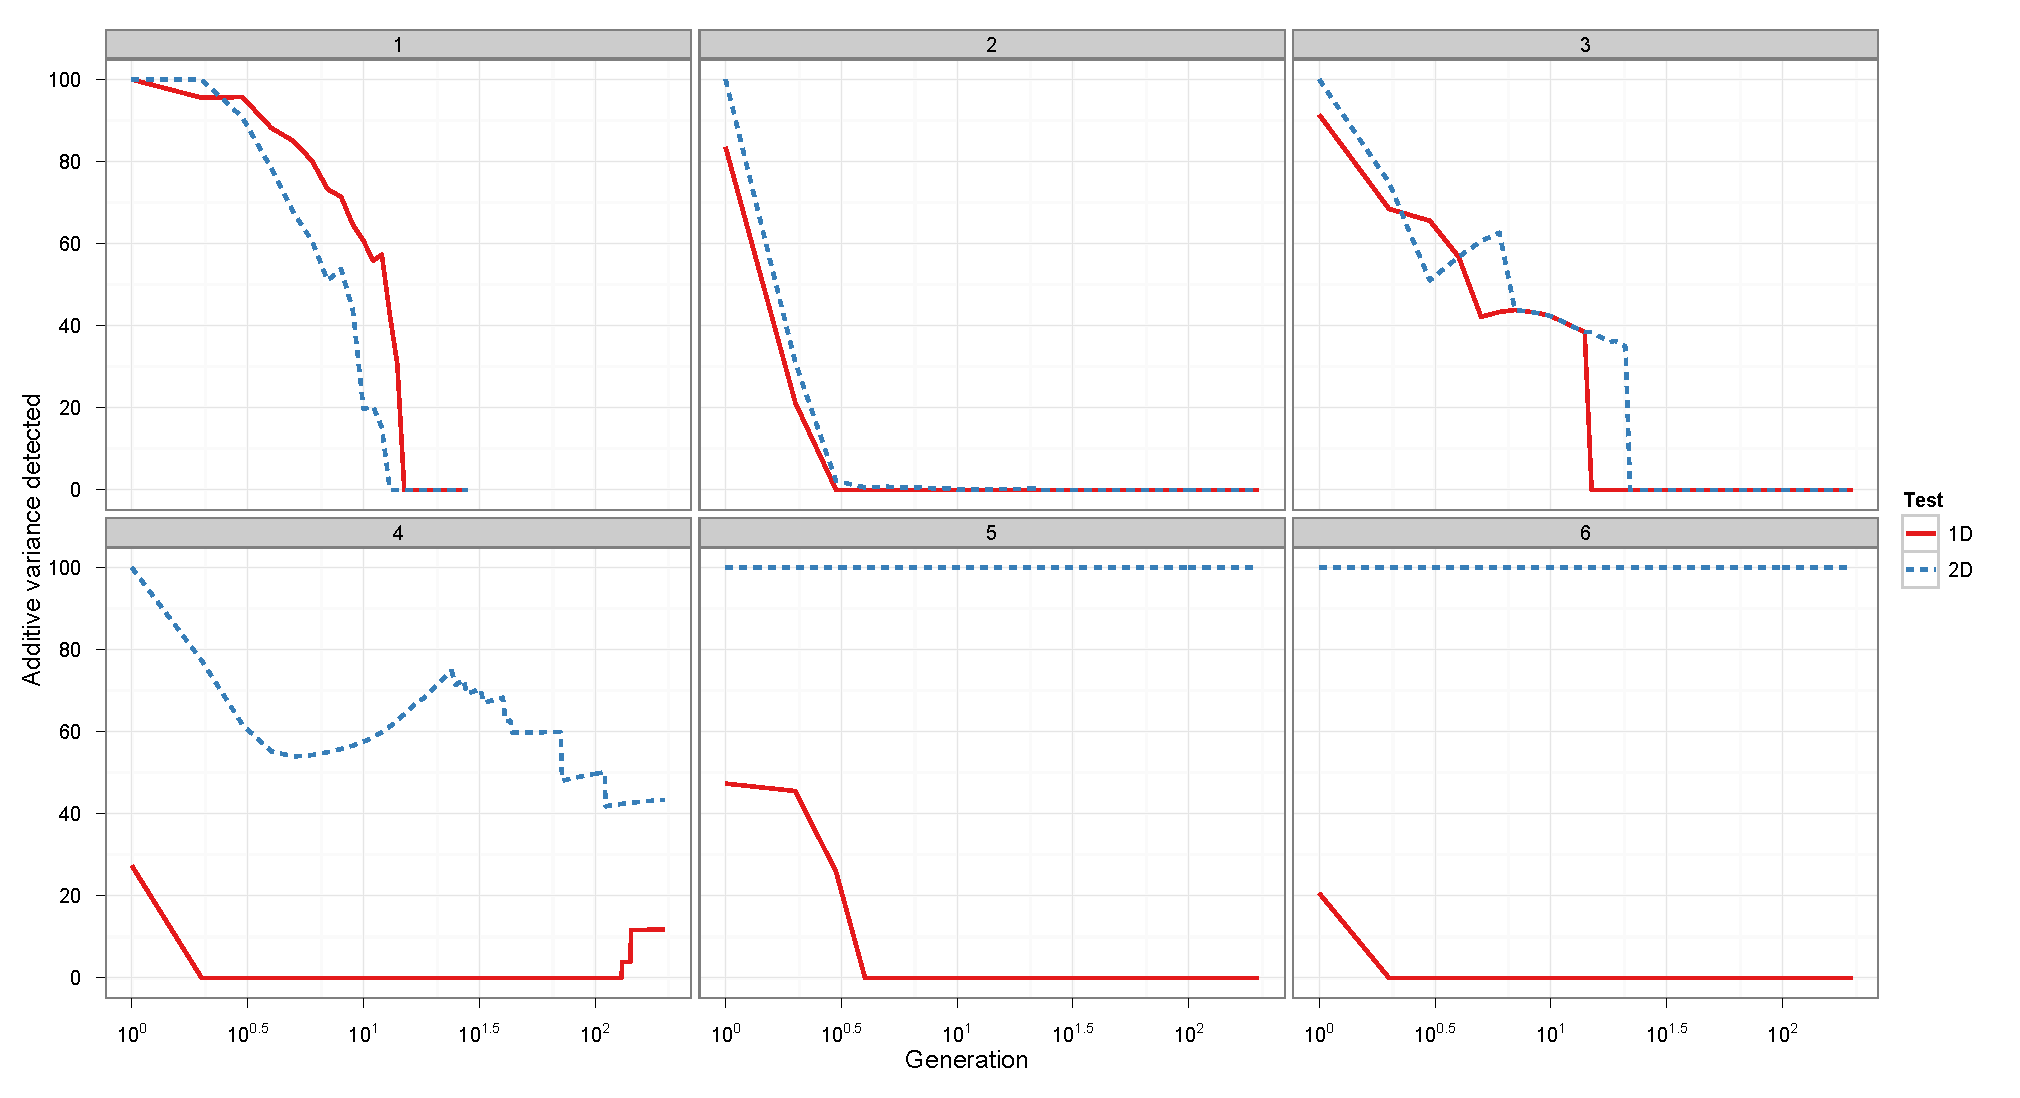
\includegraphics[width=10cm]{powersimple.pdf} \\
\end{center}
\end{frame}



\end{document}


